\section{Обзор}
В разделе сделан обзор предметной области.
Описаны скрытые марковские модели и алгоритм Витерби для работы с ними.
Приведены существующие проекты, решающие задачу гомологичности с применением скрытых марковских моделей.
Дано определение специализации.


\subsection{Скрытые марковские модели}
\label{lab:HMM}
\emph{Скрытая марковская модель}~\cite{Eddy_CHMM} (СММ) 
является дискретным вероятностным автоматом.
Модель имеет следующие параметры: множество состояний $St_{1..N}$, 
каждое из которых может создать событие из множества
$Obs_{1..K}$, вероятности $Pr\_b_{1..N}$ состояний быть
начальными, матрица $Tr$ вероятностей переходов между состояниями размера $N
\times N$ и матрица $Em$ вероятностей наблюдения события в определённом 
состоянии размера ${N \times K}$.

\subsection{Алгоритм Витерби}
\label{lab:Viterbi}
\emph{Алгоритм Витерби}~\cite{Viterbi}
(листинг~\ref{Viterbi}) считает вероятность нахождения в 
каждом состоянии СММ при условии того, что мы наблюдали последовательность событий \emph{O}.

\subsubsection{Описание методами динамического программирования}
\label{lab:dyn_Viterbi}
\begin{lstlisting}[caption=Псевдокод алгоритма Витерби, label=Viterbi, escapeinside={(*}{*)}]
function Viterbi(St, Obs, Pr_b, Tr, Em, O)
	T = length(O)
	Dp[T][N]

	for j = 1..N
		Dp[1][j] = Pr_b[j] * Em[j][O[1]]
	
	for i = 2..T
		for j = 1..N
			Dp[i][j] = 
					(*$\max_{x = 1..N}$*)(Dp[i-1][x] * Tr[x][j] * Em[j][O[i]])

	return Dp[T]
\end{lstlisting}


\subsubsection{Описание методами линейной алгебры}
\label{lab:LA_Viterbi}
Алгоритм Витерби выражается в терминах матричных 
операций из линейной алгебры~\cite{LA_Viterbi}.
Таким образом, этот алгоритм может быть реализован с 
использованием высокопроизводительных библиотек линейной 
алгебры, таких как
\name{SuiteSparse:GraphBLAS}~\cite{SuiteSparse}.

Ключевой идеей является определение специальной 
алгебраической структуры полукольцо \emph{Min\_plus} 
с операциями поэлементного сложения и умножения.
Элементы полукольца будут описывать вероятности в матрицах с
помощью дробных чисел.
Операция сложения имеет семантику взятия 
минимума из двух чисел, операция умножения --- семантику 
сложения чисел.
Нейтральным элементом по сложению будет $+\infty$, 
а по умножению 0.
Ниже приведен пример умножения матрицы на столбец 
с использованием полукольца \emph{Min\_plus}.
\[
  \begin{pmatrix}
    0 & 1 \\
    +\infty & 2
  \end{pmatrix}
  \begin{pmatrix}
    3 \\
    4
  \end{pmatrix}
  =
  \begin{pmatrix}
    min(0 + 3, 1 + 4) \\
    min(+\infty + 3, 2 + 4)
  \end{pmatrix}
  =
  \begin{pmatrix}
    3 \\
    6
  \end{pmatrix}
\]

Ко всем вероятностям в СММ применяется следующее
преобразование: отрицательный двоичный логарифм 
исходной вероятности.
Например, вероятность 0.5
будет представлена как $-1 * log_2(0.5) = 1$.
Это делается для сохранения точности расчетов.
Далее такая вероятность будет называться \emph{преобразованной}.

Для каждого события \emph{o} из множества \emph{Obs} 
определяем диагональную матрицу $P(o)$ размера $N \times N$.
Выражение $p_s(o)$ обозначает преобразованную вероятность наблюдать событие \emph{o} в состоянии \emph{s}.
\[
  P(o) =
  \begin{pmatrix}
    p_{1}(o) & \hdots & +\infty \\
    \vdots & \ddots & \vdots\\
    +\infty & \hdots & p_{N}(o)
  \end{pmatrix}
\]
Начало алгоритма Витерби --- это обработка первого события из 
последовательности \emph{O}.
В столбце \emph{Pr\_b} хранятся преобразованные вероятности 
состояний из СММ быть начальными.
Символ $\times$ обозначает умножение матриц с использованием 
полукольца \emph{Min\_plus}.
\[Probs_{1} = P(O[1]) \times Pr\_b\]
Далее вычисляются преобразованные вероятности для всех 
оставшихся событий из \emph{O}.
Матрица \emph{T} хранит преобразованные вероятности 
переходов из состояния в состояние:
\[Probs_{t} = P(O[t]) \times Tr^{T} \times Probs_{t - 1}\]
После выполнения всех шагов алгоритма, в столбце 
\emph{Probs\textsubscript{длина\_O}}
будут находиться преобразованные вероятности быть в 
определённом состоянии СММ при условии наблюдения 
последовательности событий \emph{O}.


\subsection{Существующие реализации алгоритма Витерби}
В данном разделе рассмотрены существующие высокопроизводительные реализации алгоритма Витерби, которые используются на практике.

\subsubsection{\name{HMMer}}
\name{HMMer}~\cite{HMMer} используется для поиска в базах данных 
последовательностей гомологов исследуемых протеинов, а также для создания 
профилей семейств протеинов.
Это проект с открытым исходным кодом.
Написан на языке \name{C} с возможностью использовать \name{SIMD} инструкции 
процессора.
Применяется во многих базах данных, таких как \name{Pfam}~\cite{Pfam}.

Авторами проекта были предложены вероятностные фильтры, которые используют 
\name{P7Viterbi} с частью удалённых состояний.
Применение фильтров позволяет ускорить обработку данных за счет уменьшения
вычислений в алгоритме Витерби.
Один из таких фильтров --- \name{MSV} (Multiple Segment 
Viterbi)~\cite{MSV_Eddy}.
Он моделирует последовательность из одной или более частей, 
внутри которых аминокислоты не могут быть удалены или 
вставлены.
Соответственно, веса перехода в состояния с префиксами D и I 
считаются нулевыми (рис.~\ref{MSV_example}).
\begin{figure}[t]
  \centering
  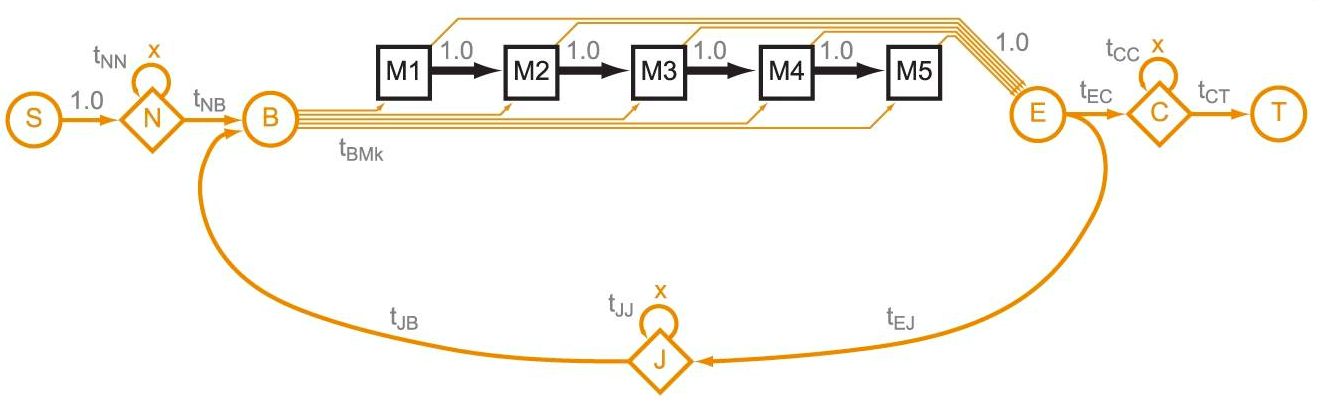
\includegraphics[width=\columnwidth]{MSV.png}
  \caption{Пример СММ вероятностного фильтра MSV~\cite{MSV_Eddy}}
  \label{MSV_example}
\end{figure}

\subsubsection{\name{CUDAMPF}}
В проекте \name{CUDAMPF}~\cite{cudampf} запрограммированы вероятностные фильтры из 
\name{HMMer} с использованием \name{CUDA}.
Код предназначен для видеокарты \name{NVIDIA} \name{Tesla K40} архитектуры
\name{Kepler}.
Проект рассчитан на определение гомологичности одновременно для множества 
протеинов.

Авторы предлагают четыре уровня параллелизма.
Первые три основаны на логическом параллелизме по данным.
Четвертый уровень использует \name{SIMD} инструкции вычислителей видеокарты.
Разделение данных по уровням позволило добиться ускорения в 23,1 раз при работе 
с фильтром \name{MSV} и в 11,6 раз с \name{P7Viterbi} по сравнению с
\name{HMMer}.

Несмотря на то, что авторами заявлена корректность реализации, в коде некорректно
вычисляется состояние E при обработке \name{P7Viterbi} и \name{MSV}.
Для этого состояния необходимо искать максимум на текущем шаге из состояний с 
префиксом M.
В исходном коде \name{CUDAMPF} переменная, хранящая максимум, 
не защищена от одновременной записи двумя или более потоками.

\subsection{Специализация}
При имеющейся программе $P$ и всех её входных параметрах 
$in$, можно получить результат выполнения $P$ на $in$.
При наличии только части параметров $in_1$ из $in$, 
\emph{специализатор} должен выполнить
вычисления и оптимизации кода в $P$, зависящие от $in_1$, 
а затем сгенерировать программу $P_{in1}$, 
которая будет принимать оставшиеся параметры $in_2$ и 
выполнять последующие вычисления (рис. \ref{spec}).
Параметры $in_1$ называются статическими, 
а $in_2$ --- динамическими.
Результат выполнения $P_{in1}$ на $in_2$ должен быть равен 
результату выполнения $P$ с параметрами $in$.
Ожидается, что специализированная программа будет 
производительнее неспециализированной версии за счет 
уменьшения вычислений или более оптимального использования 
оборудования, на котором выполняется программа.
Распространённой проблемой на практике является замедление 
производительности $P_{in1}$ из-за большого объема 
сгенерированного кода.
\begin{figure}
  \centering
  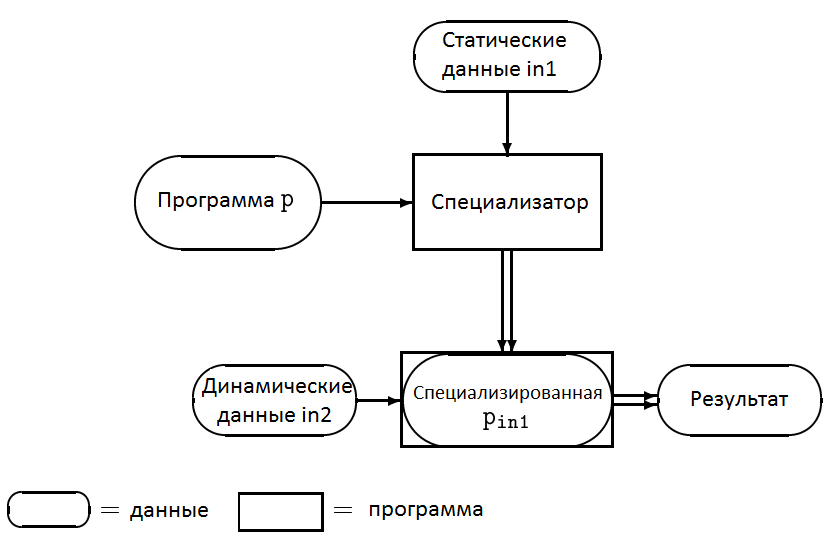
\includegraphics[width=\columnwidth]{spec.png}
  \caption{Специализация~\cite{Jones_spec}}
  \label{spec}
\end{figure}

Специализация была успешно применена в обработке 
графики~\cite{RT_spec}, обработке запросов к базам 
данных~\cite{SQL_spec} и поиску подстроки в строке на 
GPGPU~\cite{part_eval_GPU}.
Более подробно о специализации можно узнать в книге Джонса, 
Гомарда и Сестофта \cite{Jones_spec}.